\newslide{Dynamics, control and tracking}{
	\begin{columns}[c]
	\column{0.2\textwidth}
	\begin{tikzpicture}[>=latex',scale=0.4]
	\drawplanexy{-0.3}{-0.3}{-0.3}{6.7}{10}{dashed}{perception}
	
	\drawcube{0}{0}{5}{6.4}{1}{gray!40}{dinamica}{}{};
	\drawcube{0}{1.2}{5}{6.4}{1}{gray!40}{tracking}{}{};
	
	\drawcube{0}{2.4}{5}{6.4}{1}{white}{ostacoli}{}{};
	\drawcube{0}{3.6}{5}{6.4}{1}{white}{altitude}{}{};
	
	\drawcube{0}{4.8}{5}{3}{1.5}{white}{source}{}{};
	\drawcube{0}{6.5}{5}{3}{1.5}{white}{emulatore}{}{};

	\drawplanezy{3.2}{4.8}{5}{4.5}{radar_det}{fill=white,opacity=0.90}{}{};

	\drawcube{3.4}{4.8}{5}{3}{3.2}{white}{alpha}{}{};
	\drawplanexy{-0.3}{-0.3}{5.3}{6.7}{10}{dashed}{action}
	

	\draw [->,line width=1.5] (action_D) -- ++(0,0,2);
	\draw [->,line width=1.5] (perception_D) -- ++(0,0,2);

	\coordinate [at=(radar_det_D), yshift=-5] (arrows_point);
	\draw [->,dashed]  (arrows_point) -- ++(1.5,0,0); 
	\draw [->,dashed]  (arrows_point) -- ++(-1.5,0,0); 
	\end{tikzpicture}
	\vspace{6.5cm}
	\column{0.8\textwidth}
	
	\begin{block}{LQR Control}
	\centering
	\begin{tikzpicture}[auto, node distance=2cm,>=latex']
	    % Placing blocks
	    \node [block] (force) {$L_i = \dfrac{mg}{6}$};
	    \node [sum, right of=force] (sumforce) {};
	    \node [block, right of=sumforce] (hexacopter) {$\dot{\mathbf{x}}=f(\mathbf{x},\mathbf{u})$};
	    \node [block, right of=hexacopter] (integrator) {$\dfrac{1}{s}$};

	    \node [output, right of=integrator] (output) {};

	    % draw the lines
	    \draw [->] (force) -- node[pos=0.99] {} (sumforce);
	    \draw [->] (sumforce) -- node {$\mathbf{u}$} (hexacopter);
	    \draw [->] (hexacopter) -- node {} (integrator);
	    \draw [->] (integrator) -- node [name=x] {$\mathbf{x}$} (output);
	    
	    \node [sum, below of=x] (sumpos) {};
	    \node [block, right of=sumpos] (reachpoint) {$\mathbf{x}_f$};
	    \node [gain, left of=sumpos] (gain) {$K$};

	    \draw [->] (x) -- (sumpos);
	    \draw [->] (reachpoint) -- node[pos=0.99] {$-$} (sumpos);
	    \draw [->] (gain) -| node [pos=0.99] {$-$} node [pos=0.2] {$\mathbf{u}*$} (sumforce);
	    \draw [->] (sumpos) -- node {$\mathbf{e}$} (gain);
	\end{tikzpicture}	
	\end{block}
	
	\begin{block}{Newton--Euler Equations}
		\centering
		\begin{tikzpicture}
			\node (hexacopter) {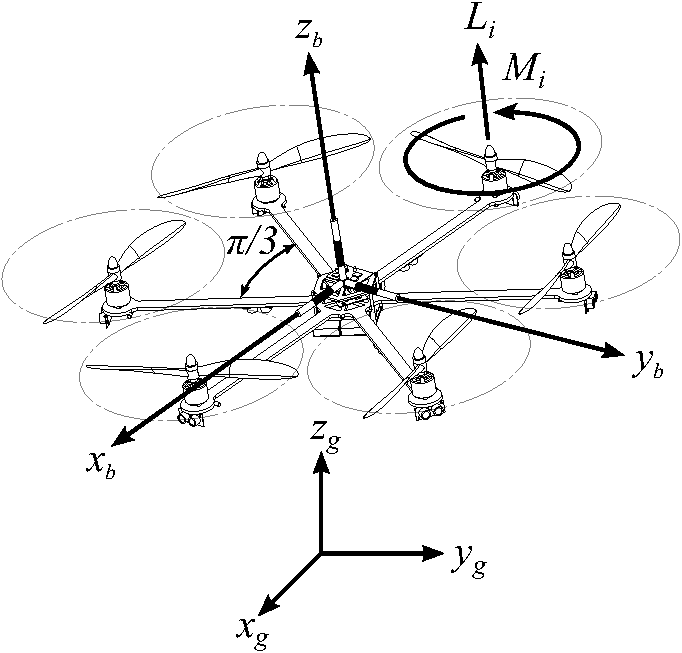
\includegraphics[height=6cm]{img/hexacopter_kine.pdf}};
			\node [right=of hexacopter] {$
				\begin{array}{rcl}
					\mathbf{x} &=& [x,y,z,\phi,\theta,\psi,u,v,w,p,q,r]^T \\
					\mathbf{u} &=& [L_i \, : \, i=1..6] \\
					\dot{\mathbf{x}} &=& f(\mathbf{x}, \mathbf{u})
				\end{array}	$};
		\end{tikzpicture}
	\end{block}
	\end{columns}
}